% Lab Writeup for HD Lab
% Adam Reyes, George Wong
% Advanced Lab Fall 2013


\documentclass[paper=a4, fontsize=11pt, abstract=on]{scrartcl} % A4 paper and 11pt font size
\usepackage[left=2.5cm,top=2.5cm,right=2.5cm,bottom=2.5cm]{geometry} 
\usepackage{amsmath}
\usepackage{graphicx}
\usepackage{sectsty}
\usepackage{fancyhdr}
\pagestyle{fancyplain}
\usepackage{parskip}
\usepackage{subcaption}
\usepackage{wrapfig}
\usepackage[english]{babel}
\usepackage{bibentry}
\usepackage {natbib}
\usepackage{float}

\numberwithin{equation}{section}
\numberwithin{figure}{section} 
\numberwithin{table}{section}
%\setlength\parindent{0pt}

\fancyhead[R]{\thepage} 
\fancyhead[L]{Reyes, Wong} 
\fancyhead[C]{M\"{o}ssbauer Effect} 
\fancyfoot[L]{} 
\fancyfoot[C]{} 
\fancyfoot[R]{} 

\newcommand{\horrule}[1]{\rule{\linewidth}{#1}}

\title{	
M\"{o}ssbauer Effect
\horrule{0.5pt}
\normalfont \normalsize 
\textsc{Advanced Experimental Physics DRAFT Report 3 }
}

\author{Adam Reyes \\ George Wong} % Your name

\date{\normalsize\today} % Today's date or a custom date


\begin{document}
\maketitle



%%%%%%%%%Abstract%%%%%%%%%%%%%%%%%%%%%
\begin{abstract}
We exploit the M\"{o}ssbauer effect of recoilless emission and
absorption to investigate the 14.4 keV excited state of iron and
measure its lifetime, $\tau$. Taking
advantage of the strong magnetic fields present in $^{57}$Fe we
observe the Zeeman splitting of the nuclear ground state and 14.4 keV
excited state of the iron nucleus.
\end{abstract}


%%%%% INTRODUCTION %%%%%
\section{Introduction}

A nucleus can absorb and emit a photon with energy corresponding to
the energy difference, E$_0$, between the ground and excited state relevant to
the transition. Due to the energy-time uncertainty relation nuclei
don't absorb and emit photons of a single energy, but a distribution
of energies centered around E$_0$, with a width of $\Gamma$. $\Gamma$
is related to the lifetime of the transition, $\tau$ by
\begin{equation}
  \label{eq:lifetime}
  \Gamma = \frac{\hbar}{\tau}.
\end{equation}
The absorption intensity of a photon by a nucleus is proportional to the photon's
energy overlap with the absorption profile of the nucleus. Therefore
$\tau$ can be calculated using eq.(\ref{eq:lifetime}) and measuring
$\Gamma$ from the energy profile of a given nucleus.

\vline

Electronic transitions in atoms are typically easy to measure due to
their relatively low energies, on the order of ~1 eV compared to
nuclear transitions on the order of ~1 keV. Because of their high
energies, free nuclei typically experience a relatively large recoil
upon emission of a photon during a transition. Nuclei emit photons on
resonance with a transition in their rest frame. During recoil a
nuclei will be moving in the opposite direction relative to the
emitted photon in the Lab-fram. As a result the emitted photon is
red-shifted off resonance in the Lab-frame, making it difficult to
measure nuclear resonant fluorescence.

\vline

In the case of a nucleus bound to a lattice, any nuclear recoil is
absorbed by the entire lattice as a phonon. Because the mass of the
lattice is much larger than the mass of an individual nucleus, the
velocity of the recoil, and hence the red-shifting away from resonance
is greatly reduced, compared to the free nucleus emission and
recoil. This ``recoil-less'' emission effect is referred to as the
M\"{o}ssbauer Effect.

\section{Stainless Steel Absorber}
\label{sec:steel}

We wish to take advantage of the M\"{o}ssbauer effect to measure the
line width, $\Gamma$ of the 14.4 keV transition of the $^{57}$Fe
nucleus. We take advantage of electron capture in a $^{57}$Co nucleus
that results in the emission of a 14.4 keV photon as a source and a
sample of stainless steel upon which to measure absorption of the 14.4
keV photon. 

\vline

In order to measure the fluorescence profile of the iron
atoms in the steel, we need to be able to sweep across resonance of
the $^{57}$Fe nuclei. To accomplish this we place the $^{57}$Co source
on an actuator that moves back and forth along the direction between
the source and absorber. Similarly to how in the case of recoil for
the free nucleus, the motion of the nuclei in the Lab-frame causes the
Lab-frame energy of the emitted photons to be shifted off resonance,
the motion of the actuator causes the 14.4 keV photons to be shifted
away from resonance, either to higher or lower energies depending on
the direction of motion. The energy shift due to this motion is given
by
\begin{equation}
  \label{eq:shift}
  \frac{\Delta E}{E} = \beta = \frac{v}{c}
\end{equation}
to first order, where $c$ is the speed of light and $\beta<<1$,  which is certainly the case for
speeds attainable in the laboratory.

\vline

The mass of the $^{57}$Co nucleus differs from that of the $^{57}$Fe
nucleus, so the resonant energies of their 14.4 keV transitions are
different. So we expect that resonant energy of the $^{57}$Fe nucleus
is not centered around exactly the same energy as the resonant
emission of the $^{57}$Co nucleus.

\subsection{Methods}
\label{sec:stmeth}

For this experiment the actuator was driven at an amplitude of 0.7
V. According to \cite{writeup} this corresponds to an amplitude of
0.508 mm. The actuator was driven by a sawtooth ramp, so for a given
frequency of modulation, $f$ and amplitude $A$,the velocity is given by
\begin{equation}
  \label{eq:vel}
  v = A\cdot f
\end{equation}

\vline

The following procedures were performed:
\begin{enumerate}
\item We did things
\end{enumerate}

\subsection{Results}
\label{sec:stres}

The data collected for the stainless steel absorber is plotted in
figure~\ref{fig:steel}. Notice that the center of resonance is off
from a velocity of 0 mm/s as we expect. We fit the data against both a lorentzian and
a gaussian to see if our data is actually representative of the
nuclear transition profile. The actual profile should be
represented by a gaussian. If there were other effects, unaccounted
for, that further spread the absorption spectrum, then the profile
would be better represented by a gaussian. We can see in
Figure~\ref{fig:steel} that our data is fit much better by the
lorentzian profile. 

\begin{figure}[h]
  \centering
  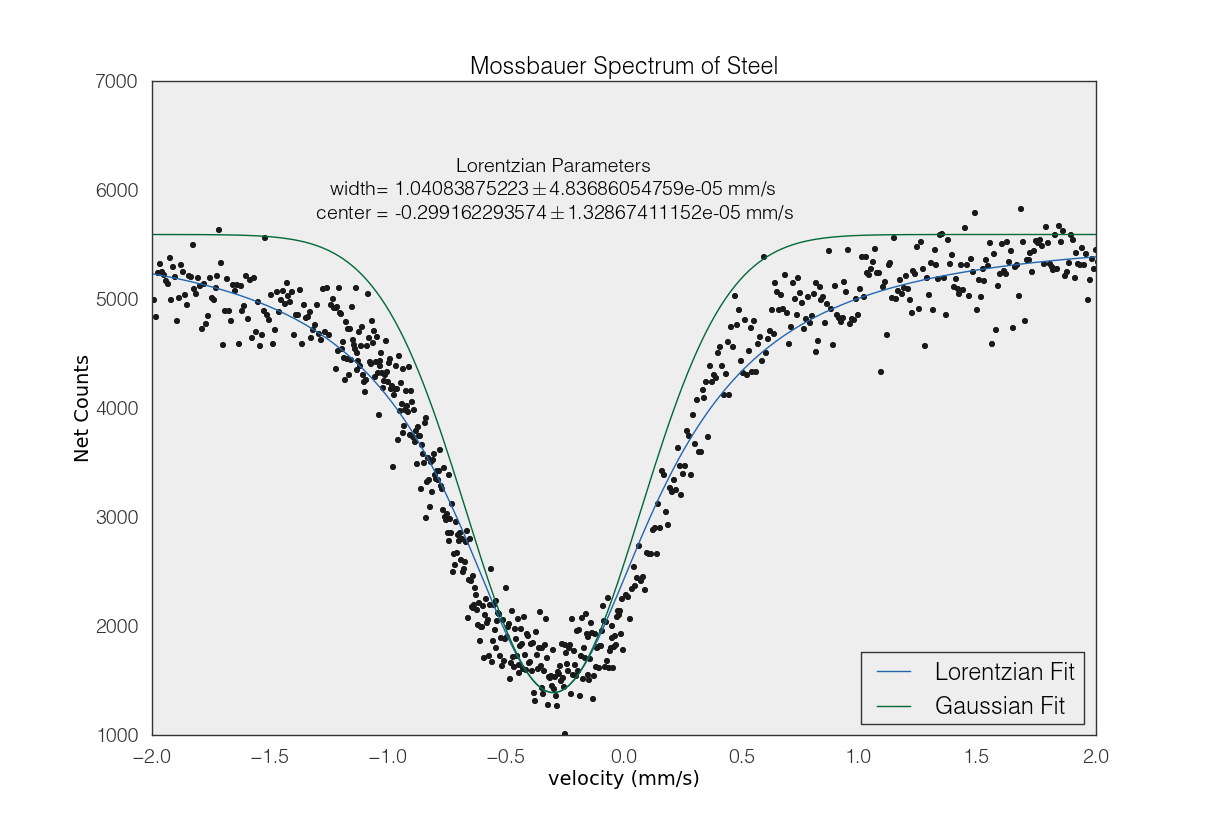
\includegraphics[width=0.9\textwidth]{steelfit}
  \caption{Data collected for the steel absorber fitted against a lorentzian and a gaussian profile.}
  \label{fig:steel}
\end{figure}

We measured a profile width of $\Delta E = 5.000 \cdot 10^{-9} \pm 0.003 \cdot 10^{-9}$ eV, which
leads to a lifetime, $\tau = 8.27 \cdot 10^{-8} \pm 0.04\cdot 10^{-8}$
s. Here our error is accounted for entirely by the fit statistics for
our data set. We are confident in this error because our data set was
taken for a fairly high resolution. Additional error, which we are not
able to quantify would arise from the discretization of intensity data
coming from the detector by the software. Further, we are limited by
the resolution and reliability of the scintillator, of which we are unsure. 


\section{$^{57}$Fe Absorber}
\label{sec:iron}

We now consider an absorber that is a sample of enriched
$^{57}$Fe. There are naturally occurring strong magnet fields within
this sample. Due to the coupling of the nuclei's magnetic moments with
these magnetic fields, called the Zeeman effect, the ground and
excited states of the nuclei are split. If we just consider the dipole
magnetic moment of the iron nuclei, then the excited stat will be
split into four levels all with equal separation, as shown in the
middle section of Figure~\ref{fig:dipsplit}.

\begin{figure}[h]
  \centering
  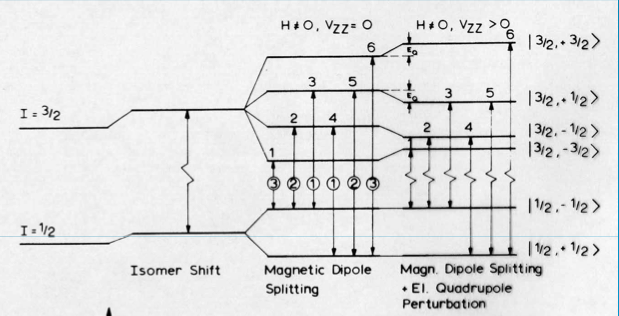
\includegraphics[width=.65\textwidth]{splits}
  \caption{Zeeman splitting due to nuclear magnetic dipole moments,
    and quadrapole moments \cite{art:slides}} 
  \label{fig:dipsplit}
\end{figure}

\vline

If we now consider the magnetic quadrapole moments, since they are not
spherically symmetric, the effect on the excited state splitting is to
space the excited states unevenly, as shown in the right side of
Figure~\ref{fig:dipsplit}. If we were to now measure the absorption
profile $^{57}$Fe, we should expect to see now the six lines depicted
in Figure~\ref{fig:dipsplit}. Further, if we can observe the
quadrapole splitting, we would expect to see a difference in the
energy splitting of the 1-2, 2-3, and 5-6 line pairs depicted in Figure~\ref{fig:dipsplit}.

\subsection{Methods}
\label{sec:irmeth}

The same procedures done for the steel absorber in
sec.~\ref{sec:steel}, but over a velocity range of -12 mm/s to +12
mm/s, in order to capture all six absorption peaks.

\subsection{Results}
\label{sec:irres}

The data collected using the iron absorber is shown in
Figure~\ref{fig:iron}. Again the data is fitted to both gaussian and
lorentzian profiles. We can again see that the data fits better to the
lorentzian profile. 

\begin{figure}[h]
  \centering
  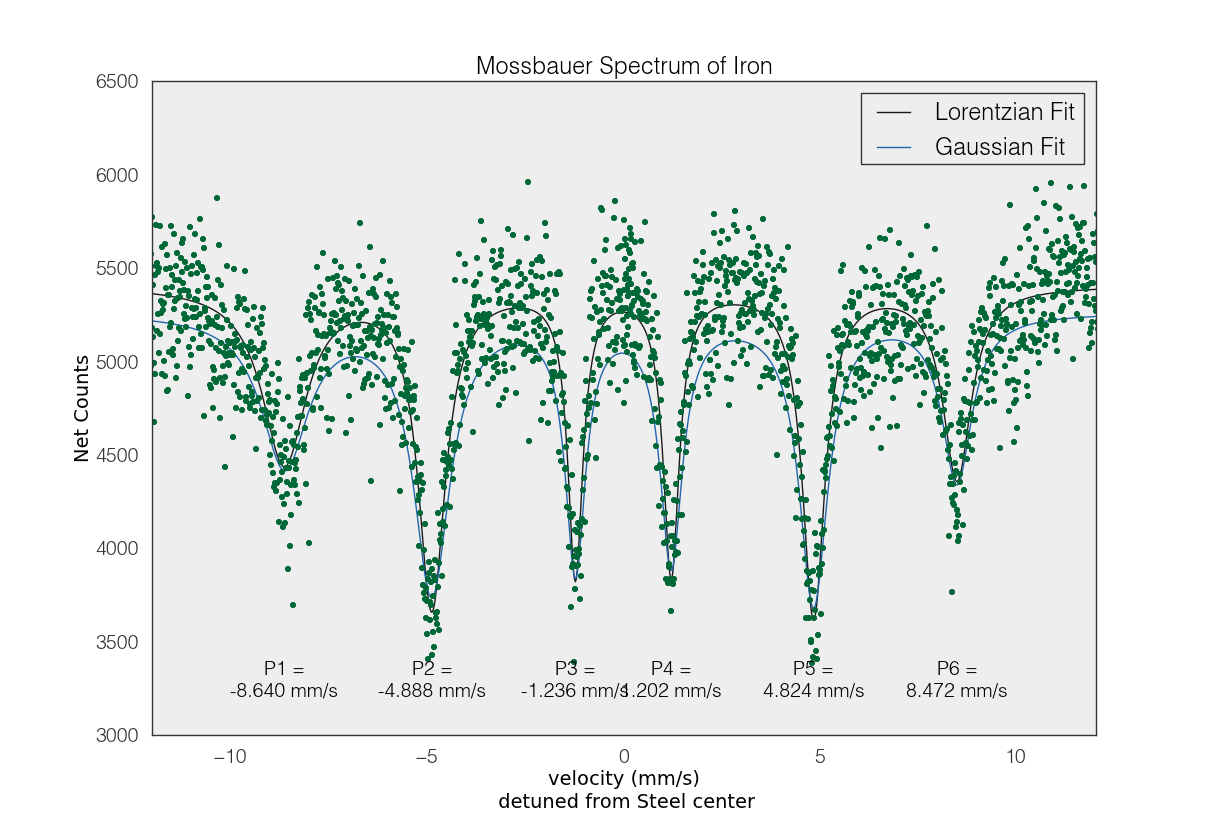
\includegraphics[width=.9\textwidth]{ironfit}
  \caption{Data collected for the $^{57}$Fe absorber, with lorentzian and gaussian fits.}
  \label{fig:iron}
\end{figure}

\begin{table}[h]
  \centering
  \begin{tabular}{r|cccccc}
       & P1 & P2 & P3 & P4 & P5 & P6 \\ \hline
    P1 & --   & \textbf{3.76}  & 7.40  & 9.84 & 13.46  & 17.10    \\
    P2 & \textbf{3.76}   & --  &  \textbf{3.65}   & 6.09  & 9.71 & 13.36   \\
    P3 & 7.40   & \textbf{3.65}   & --  & 2.44  & 6.06   & 9.71   \\
    P4 & 9.84   & 6.09   & 2.44   & -- & 3.62   & \textbf{7.27}  \\
    P5 & 13.46   & 9.71   & 6.06   & 3.62   & -- & 3.65 \\ 
    P6 & 17.10   & 13.36   & 9.71   & \textbf{7.27}   & 3.65 & --  \\
  \end{tabular}
  \caption{Peak separation data for peaks in
    Figure~\ref{fig:iron}. Given in mm/s}
  \label{tab:sep}
\end{table}

The peak separations are given in
Table~\ref{tab:sep}. We can see, as we expected that the 1-2, 2-3, and
5-6 line pairs have a different energy spacing, being evidence of
quadrapole splitting.

\appendix

\section{Macros}
\label{sec:macros}


\bibliographystyle{plain}
\bibliography{references}







\end{document}